\begin{frame}{filling buffers}
\begin{tikzpicture}
\tikzset{
    axis/.style={
        draw,ultra thick,-Latex
    },
    normal mark/.style={
        fill=black,
        alt=<5->{fill=black!50},
    },
    normal adjust/.style={
        line width=.5mm,draw=black!50!red,-Latex,
        alt=<5->{draw=black!50!red!50},
    },
}
\begin{scope}[x=1.2cm,y=1.2cm] 
    \path[fill=red!10] (5.5, 0) -- (5.0, 0) -- (0, 5) -- (0, 5.5) -- (5.5, 5.5) -- cycle;
    \path[axis] (0, 0) -- (5.5, 0)
        node[midway,below] {flow 1 bandwidth};
    \path[axis] (0, 0) -- (0, 5.5)
        node[midway,left,align=right] {flow 2\\bandwidth};
    \path[draw,dashed,very thick] (5, 0) -- (0, 5);
    \node[text=red] at (4, 4) {
        overloaded
    };
    \node[text=black,rotate=-45] at (2.25, 2.25) {
        buffers almost full
    };
    \path[draw,dotted,very thick] (4, 0) -- (0, 4);
\end{scope}
\end{tikzpicture}
\end{frame}

\begin{frame}{big buffers? (in 2011 or so)}
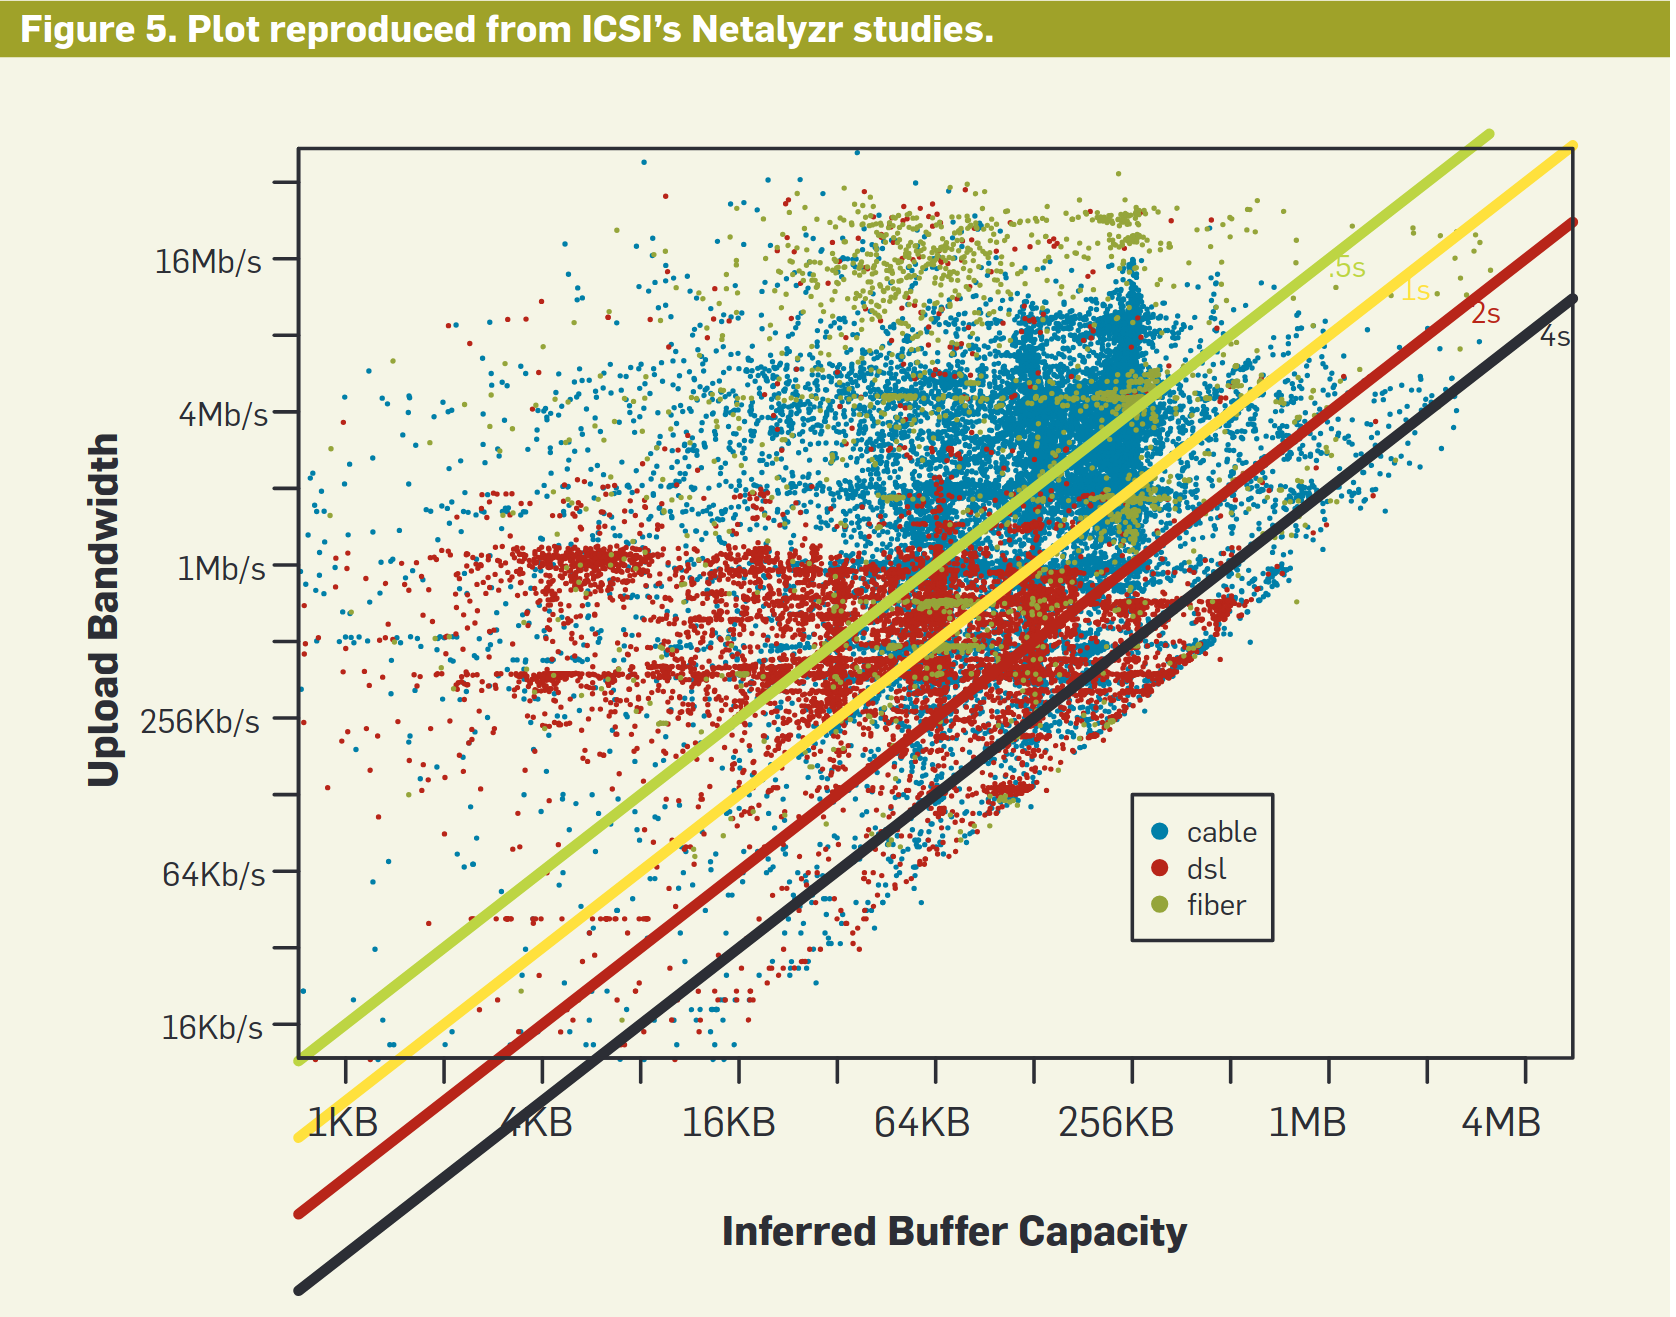
\includegraphics[width=0.6\textwidth]{../congest/cacm-bufferbloat-fig5}

{\scriptsize Jim Gettys and Kathleen Nichols, \\ ``Bufferbloat: Dark Buffers in the Internet'' (CACM, Jan 2012)}
\end{frame}

\begin{frame}{problems with big buffers}
    \begin{itemize}
    \item high latency --- bad for some applications
    \item slower response to congestion
        \begin{itemize}
        \item 1 second round trip time = 1 second to detect congestion
        \item more likely to have `congestion collapse'
        \end{itemize}
    \end{itemize}
\end{frame}

\begin{frame}{avoiding big buffers}
    \begin{itemize}
    \item multiple fixes (that can be combined):
    \vspace{.5cm}
    \item use smaller buffers?
        \begin{itemize}
        \item simpliest solution
        \end{itemize}
    \item detect congestion without full buffer\ldots
        \begin{itemize}
        \item \myemph<3>{by choosing when/which packets to drop better?}
        \item \myemph<4>{by using something other than drops?}
        \end{itemize}
    \end{itemize}
\end{frame}
